\documentclass[11pt]{charter}

% El títulos de la memoria, se usa en la carátula y se puede usar el cualquier lugar del documento con el comando \ttitle
\titulo{Red para optimización de procesos industriales} 

% Nombre del posgrado, se usa en la carátula y se puede usar el cualquier lugar del documento con el comando \degreename
\posgrado{Carrera de Especialización en Sistemas Embebidos} 
%\posgrado{Carrera de Especialización en Internet de las Cosas} 
%\posgrado{Carrera de Especialización en Intelegencia Artificial}
%\posgrado{Maestría en Sistemas Embebidos} 
%\posgrado{Maestría en Internet de las cosas}

% Tu nombre, se puede usar el cualquier lugar del documento con el comando \authorname
\autor{Ing. Federico Meghinasso} 

% El nombre del director y co-director, se puede usar el cualquier lugar del documento con el comando \supname y \cosupname y \pertesupname y \pertecosupname
\director{Esp. Ing. Pablo Slavkin}
\pertenenciaDirector{Novospace} 
% FIXME:NO IMPLEMENTADO EL CODIRECTOR ni su pertenencia
\codirector{} % si queda vacio no se deberíá incluir 
\pertenenciaCoDirector{}

% Nombre del cliente, quien va a aprobar los resultados del proyecto, se puede usar con el comando \clientename y \empclientename
\cliente{Ricardo Meghinasso }
\empresaCliente{Industrias Meghinasso S.A. }

% Nombre y pertenencia de los jurados, se pueden usar el cualquier lugar del documento con el comando \jurunoname, \jurdosname y \jurtresname y \perteunoname, \pertedosname y \pertetresname.
\juradoUno{Nombre y Apellido (1)}
\pertenenciaJurUno{pertenencia (1)} 
\juradoDos{Nombre y Apellido (2)}
\pertenenciaJurDos{pertenencia (2)}
\juradoTres{Nombre y Apellido (3)}
\pertenenciaJurTres{pertenencia (3)}
 
\fechaINICIO{2 de marzo de 2021}		%Fecha de inicio de la cursada de GdP \fechaInicioName
\fechaFINALPlanificacion{20 de abril de 2021} 	%Fecha de final de cursada de GdP
\fechaFINALTrabajo{2 de marzo de 2022}		%Fecha de defensa pública del trabajo final


\begin{document}

\maketitle
\thispagestyle{empty}
\pagebreak


\thispagestyle{empty}
{\setlength{\parskip}{0pt}
\tableofcontents{}
}
\pagebreak


\section{Registros de cambios}
\label{sec:registro}


\begin{table}[ht]
\label{tab:registro}
\centering
\begin{tabularx}{\linewidth}{@{}|c|X|c|@{}}
\hline
\rowcolor[HTML]{C0C0C0} 
Revisión & \multicolumn{1}{c|}{\cellcolor[HTML]{C0C0C0}Detalles de los cambios realizados} & Fecha      \\ \hline
1.0      & Creación del documento                                          & 2/03/2021 \\ \hline
1.1      & Se completó hasta el punto 5 inclusive & 15/03/2021 \\ \hline
1.2      & Se corrigió la descripción técnica\newline
           Se terminó el punto 6\newline
           Se agregaron historias de usuario & 23/03/2021 \\ \hline
1.3      & Se agregó hasta el punto 11      & 30/03/2021  \\ \hline
1.4     & Se agregó hasta el punto 17       & 6/4/2021 \\ \hline
1.5     & Se hicieron correcciones y se agregó el director       & 13/4/2021 \\ \hline
\end{tabularx}
\end{table}

\pagebreak



\section{Acta de constitución del proyecto}
\label{sec:acta}

\begin{flushright}
Buenos Aires, \fechaInicioName
\end{flushright}

\vspace{2cm}

Por medio de la presente se acuerda con el Ing. \authorname\hspace{1px} que su Trabajo Final de la \degreename\hspace{1px} se titulará ``\ttitle'', consistirá esencialmente en el prototipo preliminar de una red de nodos, cada uno con una función específica, para reducir los tiempos muertos y mejorar el flujo de información dentro de una industria, y tendrá un presupuesto preliminar estimado de 600 hs de trabajo y u\$s 9035, con fecha de inicio \fechaInicioName\hspace{1px} y fecha de presentación pública \fechaFinalName.

Se adjunta a esta acta la planificación inicial.

\vfill

% Esta parte se construye sola con la información que hayan cargado en el preámbulo del documento y no debe modificarla
\begin{table}[ht]
\centering
\begin{tabular}{ccc}
\begin{tabular}[c]{@{}c@{}}Ariel Lutenberg \\ Director posgrado FIUBA\end{tabular} & \hspace{2cm} & \begin{tabular}[c]{@{}c@{}}\clientename \\ \empclientename \end{tabular} \vspace{2.5cm} \\ 
\multicolumn{3}{c}{\begin{tabular}[c]{@{}c@{}} \supname \\ Director del Trabajo Final\end{tabular}} \vspace{2.5cm} \\
%\begin{tabular}[c]{@{}c@{}}\jurunoname \\ Jurado del Trabajo Final\end{tabular}     &  & \begin{tabular}[c]{@{}c@{}}\jurdosname\\ Jurado del Trabajo Final\end{tabular}  \vspace{2.5cm}  \\
%\multicolumn{3}{c}{\begin{tabular}[c]{@{}c@{}} \jurtresname\\ Jurado del Trabajo Final\end{tabular}} \vspace{.5cm}                                                                     
\end{tabular}
\end{table}




\section{Descripción técnica-conceptual del proyecto a realizar}
\label{sec:descripcion}

%Hoy en día la industria se enfrenta a lo que se denomina la cuarta revolución industrial o industria 4.0\footnote{\url{https://es.wikipedia.org/wiki/Industria_4.0}} proponiendo lo que se conoce como ``fábricas inteligentes''. Para ello es necesario un flujo constate de información entre todos los sectores que componen una industria aumentando la eficiencia en la toma de decisiones.  

\empclientename es una empresa que se dedica a la fabricación de elementos para la conexión de agua domiciliaria a la red de agua pública con la marca Bronzo Aleaciones. La mayor parte de sus productos se realizan en latón. El proceso de fabricación dentro de la empresa incluye fundición, inyección, mecanizado y armado.

Este proyecto se propone introducir a \empclientename a la industria 4.0\footnote{\url{https://es.wikipedia.org/wiki/Industria_4.0}} con el objetivo de convertirla en lo que se conoce como una ``fábrica inteligente''. Para ello se propone una red como la que se observa en la figura \ref{fig:DiagramaRed} con el objetivo de lograr un flujo constante de la información y descentralizar la toma de decisiones.



%El objetivo del proyecto es mejorar el control de \textit{stock}, obtener métricas más precisas de los desperdicios a lo largo del proceso de fabricación y reducir los tiempos muertos. Para esto se plantea el desarrollo de una serie de dispositivos que se conecten a una red que permita enviar alertas de estado y a su vez avisarle a quien corresponda para que esa alerta sea atendida. En la figura \ref{fig:DiagramaRed} se puede ver un diagrama de la red propuesta. 

\begin{figure}[H]
    \centering
    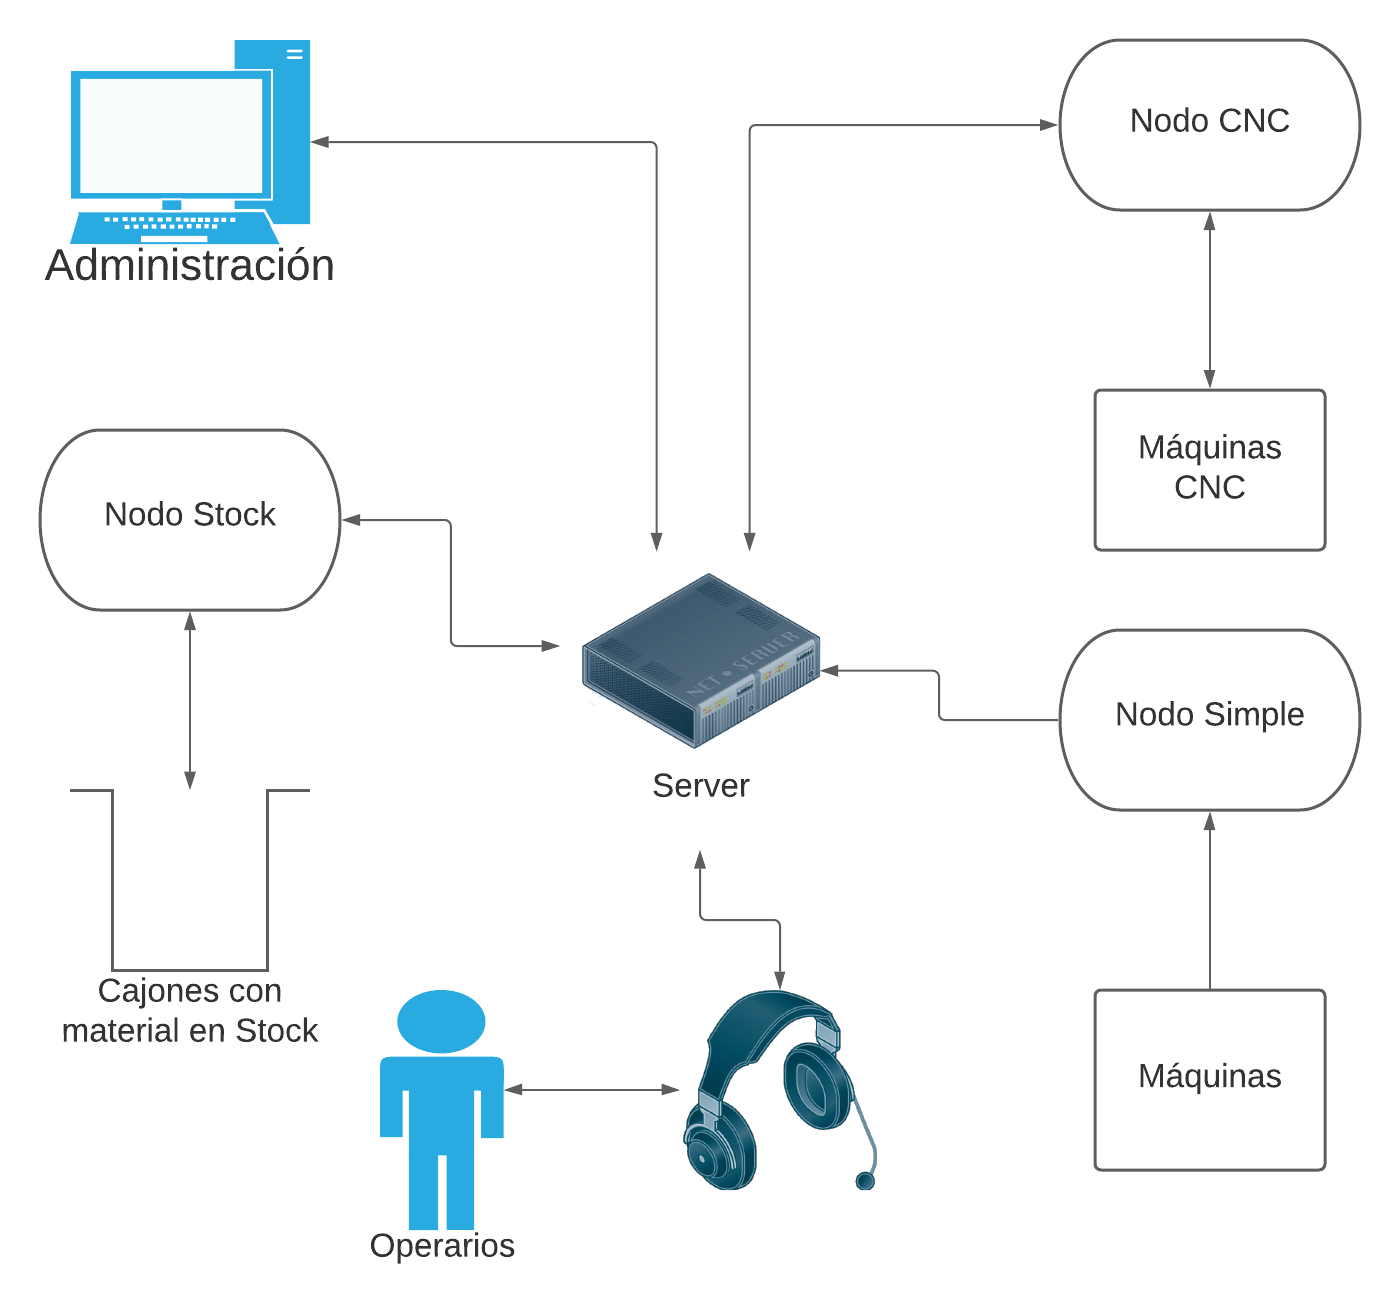
\includegraphics[scale=0.5]{Figuras/diagBloquesRed.png}
    \caption{Diagrama de la red propuesta con sus diferentes dispositivos.}
    \label{fig:DiagramaRed}
\end{figure}

La red consistirá de un servidor y cuatro tipos diferentes de nodos:
\begin{itemize}
    \item Los nodos simples son aquellos que se conectarán a las máquinas que tienen ciclos de trabajo que no precisan de un operario para funcionar, sino que solo requieren de su atención para la carga y descarga de la misma y el reinicio del ciclo. Estos nodos deberán generar tres tipos de alerta: alarma, máquina en operación y fin de ciclo. Estas serán enviadas al servidor.
    \item Los nodos CNC tendrán las mismas funciones que los nodos simples y, además, se le agregarán una comunicación serie mediante un puerto RS-232 para poder cargar y descargar los programas de las máquinas. Los programas se gestionarán desde la administración a través del servidor.
    \item Los nodos de \textit{stock} tendrán que medir cuan llenos están los cajones con piezas y enviar este dato al servidor periódicamente. Cuando los cajones estén por debajo de un límite tendrán que mandar una alerta al servidor y encender un led indicador. Este límite se tendrá que poder configurar desde la administración a través del servidor. 
    \item Los nodos de los operarios solo recibirán alertas provenientes del servidor. Las alertas les tendrán que indicar qué es lo que tienen que hacer. 
\end{itemize}
El servidor tendrá dos tareas principales. Por un lado, se tendrá que encargar de llevar un \textit{stock} aproximado en planta de las diferentes piezas en sus diferentes estados de procesamiento. Y, por otro, tendrá que controlar el estado en el que se encuentran las máquinas en planta para que cuando una necesite ser atendida, este asigne la tarea automáticamente a un operario. La asignación de tareas en función de las máquinas, los parámetros para calcular el \textit{stock} y las alturas mínimas de los cajones tienen que poder configurarse desde la administración.     


\section{Identificación y análisis de los interesados}
\label{sec:interesados}

\begin{table}[ht]
%\caption{Identificación de los interesados}
%\label{tab:interesados}
\begin{tabularx}{\linewidth}{@{}|l|X|X|l|@{}}
\hline
\rowcolor[HTML]{C0C0C0} 
Rol           & Nombre y Apellido & Organización 	& Puesto 	\\ \hline
Cliente       & \clientename      &Industrias\newline Meghinasso S.A.	& Gerente general 	\\ \hline
Responsable   & \authorname       & Industrias\newline Meghinasso S.A. 	& Ingeniero de Desarrollo 	\\ \hline
Colaboradores & Matias Meghinasso & Industrias\newline Meghinasso S.A. 	&  Ingeniero de Desarrollo \\ \hline
Orientador    & \supname	      & \pertesupname 	& Director	Trabajo final \\ \hline
Usuario final & Operarios,\newline
                jefe de fábrica,
                personal\newline administrativo & Industrias\newline Meghinasso S.A. & - \\ \hline
\end{tabularx}
\end{table}



\section{1. Propósito del proyecto}
\label{sec:proposito}

El propósito de este proyecto es desarrollar todos los dispositivos esenciales para implementar una red industrial que ayude a bajar los tiempos muertos y mejorar los controles de \textit{stock} en la planta industrial de Industrias Meghinasso S.A. 

\section{2. Alcance del proyecto}
\label{sec:alcance}

El presente proyecto incluye:
\begin{itemize}
    \item Prototipo funcional de cada nodo.
    \item Prototipo funcional del servidor.
    \item Desarrollo y documentación del firmware necesario.
    \item Desarrollo de la interfaz de usuario.
    \item Pruebas de validación y verificación.
\end{itemize}

El presente proyecto no incluye:
\begin{itemize}
    \item Desarrollo de los PCB finales. Se utilizarán las placas de desarrollo a elegir.
\end{itemize}


\section{3. Supuestos del proyecto}
\label{sec:supuestos}
Para el desarrollo del presente proyecto se supone que:
\begin{itemize}
    \item Los fondos necesarios para el proyecto están disponibles.
    \item Los materiales necesarios serán adquiridos en tiempo y forma.
    \item El tiempo disponible será suficiente para el desarrollo del proyecto.
\end{itemize}


\section{4. Requerimientos}
\label{sec:requerimientos}

\begin{enumerate}
    \item Requerimientos generales:
    \begin{enumerate}
        \item Los nodos deben ser grado IP64.
        \item La comunicación entre el servidor y los nodos debe ser inalámbrica.
        \item La documentación del proyecto debe seguirse con control de versiones GIT. 
    \end{enumerate}
    \item Requerimientos del servidor:
    \begin{enumerate}
        \item Se tiene que conectar a la red LAN de la fábrica mediante WiFi/Ethernet.
        \item Debe tener una interfaz para poder configurar la asignación de tareas según la máquina, los parámetros para calcular el \textit{stock} y las alturas mínimas de los cajones de piezas. Además, se deben poder configurar los parámetros de la comunicación serie de los nodos CNC.
        \item El tiempo máximo entre consultas para los nodos comunes y CNC tiene que ser de 60 segundos.
        \item El tiempo máximo entre que se recibe una alerta de una máquina y se le asigna a un operario para que la atienda no puede superar los 10 segundos. 
    \end{enumerate}
    \item Requerimiento de los nodos comunes:
    \begin{enumerate}
        \item Deben tener entradas digitales opto-acopladas para poder leer las alarmas y las alertas de las máquinas. Estas señales son salidas de PLC de 24V DC.
    \end{enumerate}
    \item Requerimientos de los nodos CNC:
    \begin{enumerate}
        \item Deben tener entradas digitales opto-acopladas para leer señales de alarma, en proceso y fin de ciclo. Estas señales son salidas de PLC de 24V DC.
        \item Deben poder subir y bajar archivos mediante una comunicación serie utilizando un puerto RS-232. La configuración va a depender del controlador de la máquina. Actualmente \empclientename cuenta con controles de las marcas Fanuc y Siemens en sus equipos.
    \end{enumerate}
    \item Requerimientos de los nodos de control de \textit{stock}:
    \begin{enumerate}
        \item Deben medir la altura de piezas de los cajones que tienen 45 cm de altura. 
        \item Deben generar alertas cuando la altura sea menor a la configurada.
    \end{enumerate}
    \item Requerimientos de los nodos para el personal:
    \begin{enumerate}
        \item Deben poder recibir alertas.
        \item Deben poder indicar qué generó la alerta.
        \item Deben estar alimentado por una batería recargable de litio de 3.7 V con la capacidad necesaria para alimentar el nodo durante 6 jornadas laborales de 9 hs sin ser recargada.
    \end{enumerate}
\end{enumerate}


\section{Historias de usuarios (\textit{Product backlog})}
\label{sec:backlog}

Para analizar las historias de usuarios se utilizara el siguiente criterio:
\renewcommand{\theenumi}{\Alph{enumi}}
\begin{enumerate}
    \item Cantidad de trabajo a realizar
    \begin{itemize}
        \item Bajo: 1
        \item Medio: 5
        \item Alto: 13
    \end{itemize}
    \item Complejidad del trabajo a realizar
    \begin{itemize}
        \item Bajo: 1
        \item Medio: 3
        \item Alto: 8
    \end{itemize}
    \item Incertidumbre del trabajo a realizar
    \begin{itemize}
        \item Bajo: 1
        \item Medio: 2
        \item Alto: 3
    \end{itemize}
\end{enumerate}

Se analizaron las siguientes historias:

\renewcommand{\theenumi}{\arabic{enumi}}
\begin{enumerate}
    \item Como gerente de compras quiero saber el nivel de \textit{stock} que hay en planta para poder programar la compra de materia prima. 
    \begin{itemize}
        \item A: 13
        \item B: 3
        \item C: 1
    \end{itemize}
    \textit{Storypoints}:21
    \item Como jefe de fábrica quiero saber los niveles de \textit{stock} en sus diferentes estados de procesamiento para mejorar la programación de la producción.
    \begin{itemize}
        \item A: 13
        \item B: 8
        \item C: 1
    \end{itemize}
    \textit{Storypoints}:34
    \item Como jefe de fábrica quiero saber que máquinas están desocupadas para asignarles una tarea lo antes posible. 
    \begin{itemize}
        \item A: 5
        \item B: 8
        \item C: 3
    \end{itemize}
    \textit{Storypoints}:21
    \item Como operario quiero saber cuando una de las máquinas de las que soy responsable termina su trabajo para volverla a ponerla a trabajar en el menor tiempo posible. 
    \begin{itemize}
        \item A: 5
        \item B: 3
        \item C: 3
    \end{itemize}
    \textit{Storypoints}:13
    \item Como jefe de despacho quiero asegurarme que voy a tener todas las piezas necesarias para armar los pedidos. 
    \begin{itemize}
        \item A: 5
        \item B: 3
        \item C: 1
    \end{itemize}
    \textit{Storypoints}:13
\end{enumerate}


\section{5. Entregables principales del proyecto}
\label{sec:entregables}

\begin{itemize}
    \item El servidor funcionando
    \item Un nodo de cada tipo mencionado funcionando.
    \item Manual de uso
    \item Código fuente
    \item Informe final
\end{itemize}


\section{6. Desglose del trabajo en tareas}
\label{sec:wbs}

\begin{enumerate}
    \item Análisis del proyecto \textbf{(40 hs)}
    \begin{enumerate}
        \item Definir el alcance del proyecto. (20 hs)
        \item Planificación. (14 hs)
        \item Búsqueda de información de comunicaciones inalámbricas en ambientes industriales. (6 hs)
    \end{enumerate}
    \item Definiciones generales del proyecto \textbf{(60 hs)}
    \begin{enumerate}
        \item Definir la arquitectura de la red. (18 hs)
        \item Definir el protocolo de comunicación. (16 hs)
        \item Definir la arquitectura de la interfaz de usuario. (12 hs)
        \item Definir método para realizar la medición de la altura de piezas en los cajones. (10 hs)
        \item Documentación. (4 hs)
    \end{enumerate}
    \item Diseño y armado del hardware - Servidor \textbf{(70 hs)}
    \begin{enumerate}
        \item Estudio y selección de arquitectura. (30 hs)
        \item Selección de componentes. (20 hs)
        \item Adquisición de componentes. (4 hs)
        \item Pruebas iniciales de funcionamiento. (12 hs)
        \item Documentación. (4 hs)
    \end{enumerate}
    \item Diseño y armado del hardware - Nodos \textbf{(70 hs)}
    \begin{enumerate}
        \item Estudio y selección de arquitectura. (30 hs)
        \item Selección de componentes. (20 hs)
        \item Adquisición de componentes. (4 hs)
        \item Pruebas iniciales de funcionamiento. (12 hs)
        \item Documentación. (4 hs)
    \end{enumerate}
    \item Desarrollo del firmware \textbf{(180 hs)}
    \begin{enumerate}
        \item Comunicación del servidor con la red LAN de la fábrica. (45 hs)
        \item Interfaz de usuario del servidor. (45 hs)
        \item Comunicación de los nodos con el servidor. (20 hs)
        \item Generación de alertas de alarma, máquina en operación y fin de ciclo de los nodos comunes y CNC. (20 hs)
        \item Comunicación serie mediante puerto RS-232 en los nodos CNC. (20 hs)
        \item Alertas sonoras en los nodos de los operarios. (16 hs)
        \item Medición de la altura de piezas en los nodos de \textit{stock}. (10 hs)
        \item Documentación. (4 hs)
    \end{enumerate}
    \item Verificación \textbf{(100 hs)}
    \begin{enumerate}
        \item Verificación de la comunicación serie de los nodos CNC. (30 hs)
        \item Verificación del tiempo máximo de consulta de los nodos comunes y CNC. (24 hs)
        \item Verificación del tiempo máximo desde que el servidor recibe una alerta hasta que se asigna un operario para que la atienda. (22 hs)
        \item Verificación de la medición de altura de los nodos de \textit{stock}. (20 hs)
        \item Documentación. (4 hs)
    \end{enumerate}
    \item Documentación \textbf{(80 hs)}
    \begin{enumerate}
        \item Manual de uso. (16 hs)
        \item Memoria del trabajo final. (52 hs)
        \item Presentación final. (12 hs)
    \end{enumerate}
\end{enumerate}

Cantidad total de horas: 600 hs.



\section{7. Diagrama de Activity On Node}
\label{sec:AoN}

\begin{figure}[htpb]
\centering 
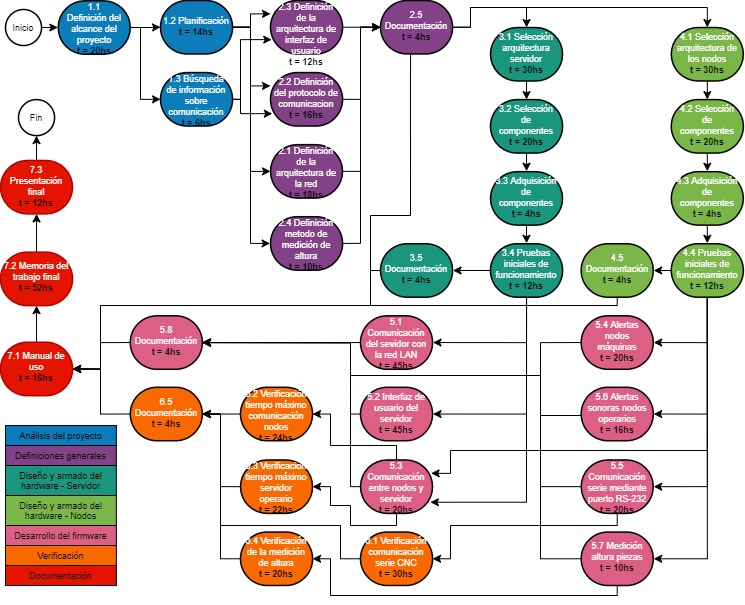
\includegraphics[width=\textwidth]{./Figuras/AoN-Plan de Proyecto.jpg}
\caption{Diagrama en \textit{Activity on Node}}
\label{fig:AoN}
\end{figure}
\newpage

\section{8. Diagrama de Gantt}
\label{sec:gantt}
\begin{figure}[htpb]
\centering 
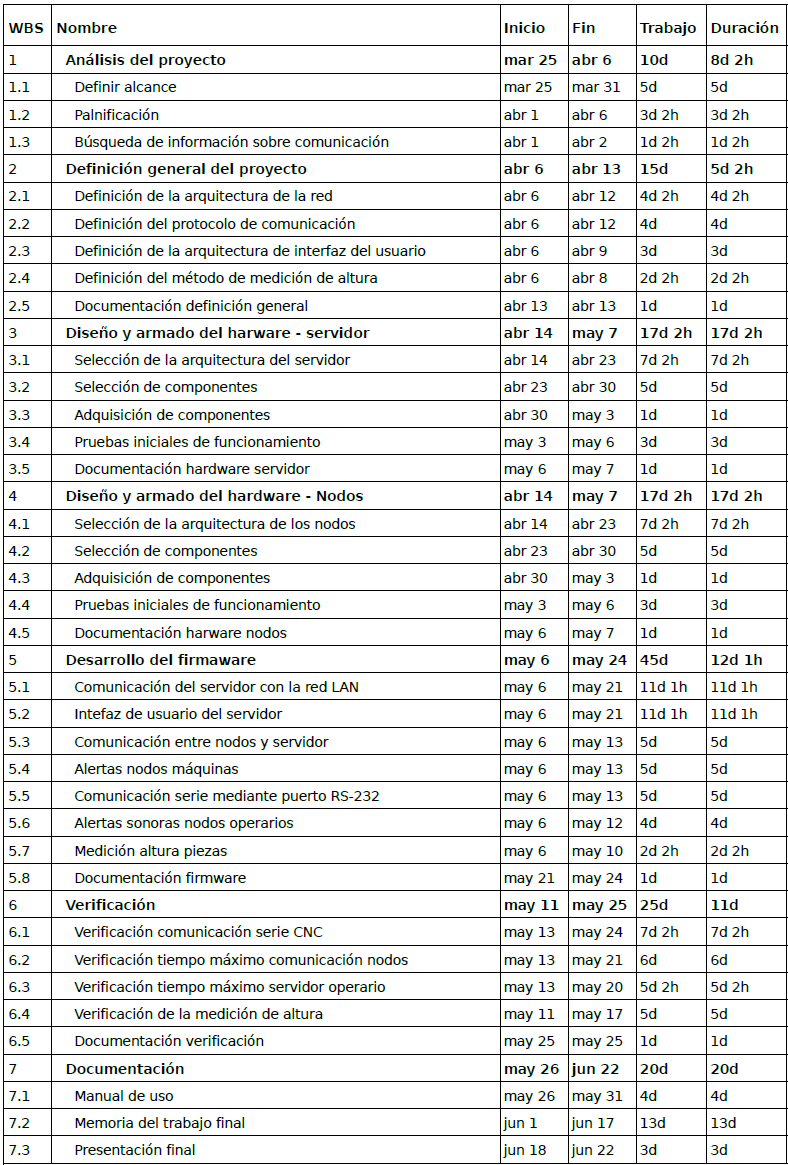
\includegraphics[scale=0.7]{Figuras/tareasGantt.png}
\caption{Tabla de tareas del diagrama de gantt}
\label{fig:tareasGantt}
\end{figure}

\begin{landscape}
\begin{figure}[htpb]
\centering 
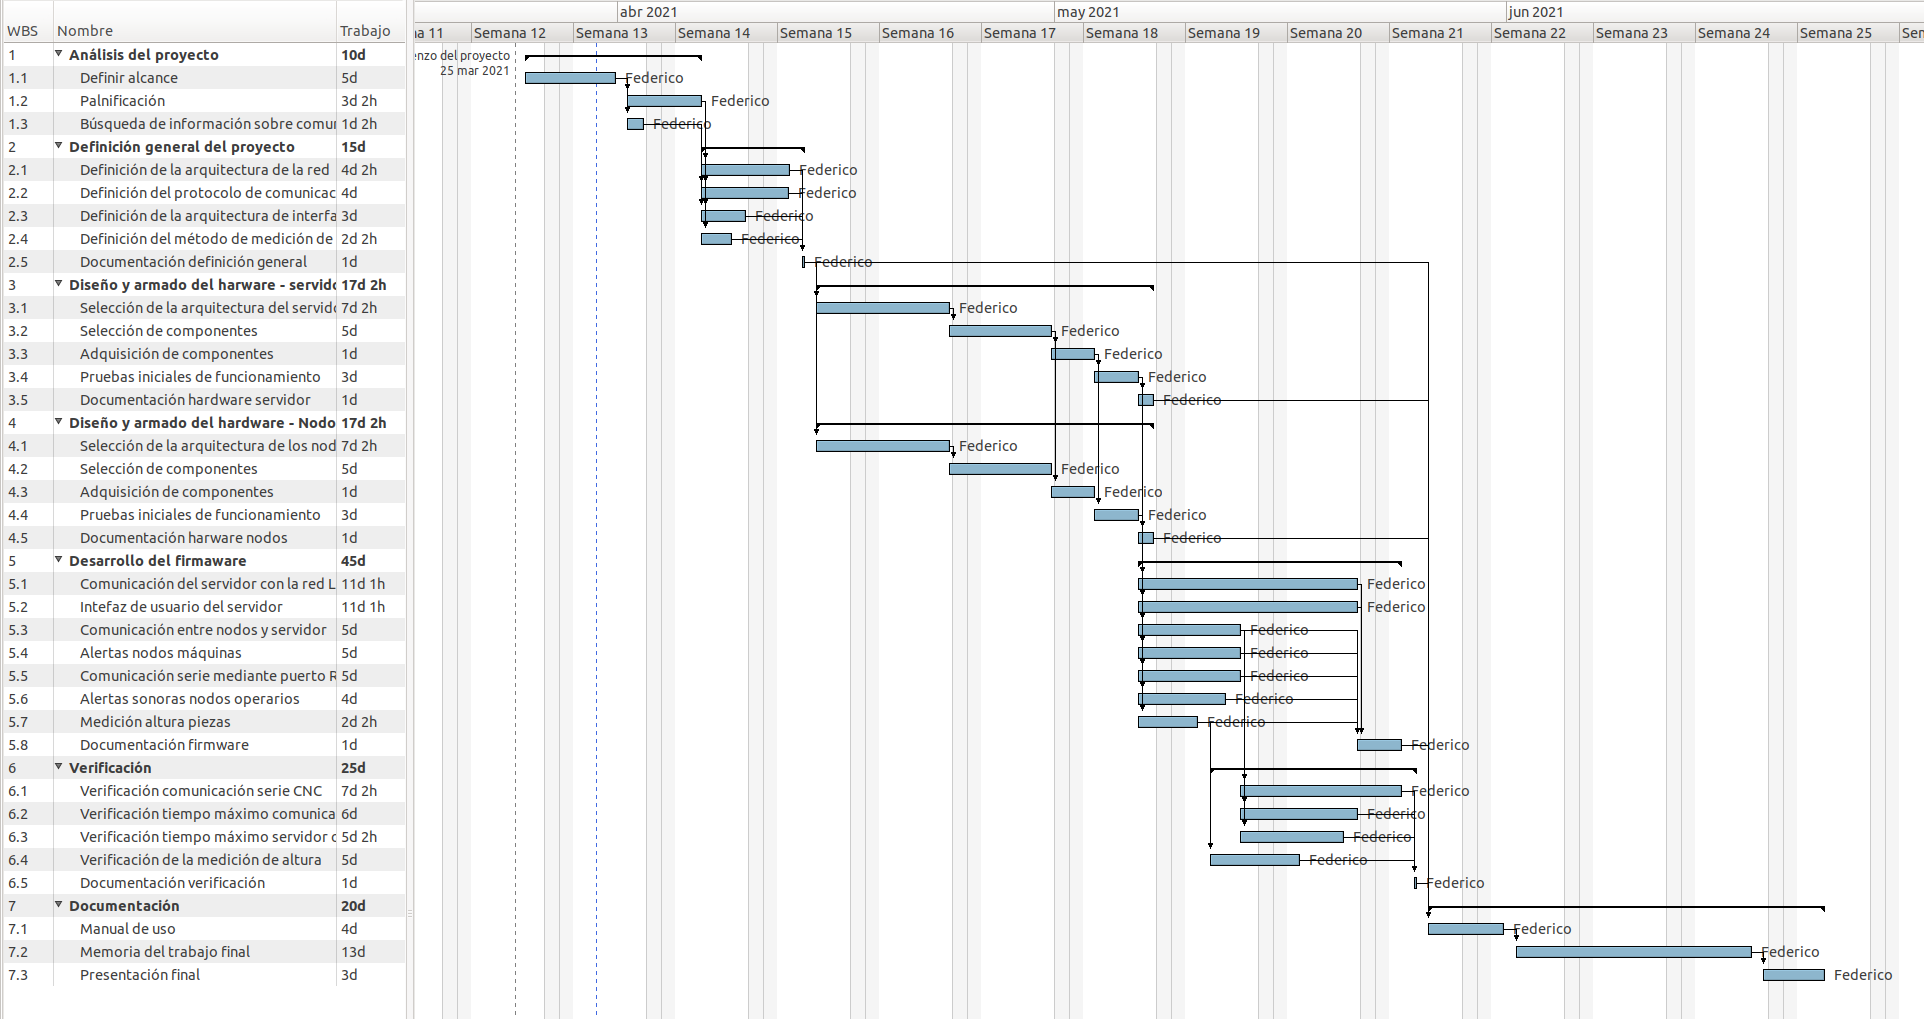
\includegraphics[scale=0.6]{Figuras/gantt.png}
\caption{Diagrama de \textit{gantt}}
\label{fig:gantt}
\end{figure}
\end{landscape}



\section{9. Matriz de uso de recursos de materiales}
\label{sec:recursos}


\begin{table}[H]
\label{tab:recursos}
\centering
\begin{tabular}{|c|c|c|c|c|}
\hline
\cellcolor[HTML]{C0C0C0} & \cellcolor[HTML]{C0C0C0} & \multicolumn{3}{c|}{\cellcolor[HTML]{C0C0C0}Recursos requeridos (horas)} \\ \cline{3-5} 
\multirow{-2}{*}{\cellcolor[HTML]{C0C0C0}\begin{tabular}[c]{@{}c@{}}Código\\ WBS\end{tabular}} & \multirow{-2}{*}{\cellcolor[HTML]{C0C0C0}\begin{tabular}[c]{@{}c@{}}Nombre \\ tarea\end{tabular}} & Computadora & Placa desarrollo & Lab. Electrónica \\ \hline
1 & Análisis del proyecto & 40 &  & \\ \hline
2 & Definiciones generales & 60 & & \\ \hline
3.1 - 3.3 & Diseño y armado servidor & 54 & & \\ \hline
3.4 & Pruebas iniciales & 12 & 12 & 12 \\ \hline
3.5 & Documentación & 4 & & \\ \hline
4.1 - 4.3 & Diseño y armado servidor & 54 & & \\ \hline
4.4 & Pruebas iniciales & 12 & 12 & 12 \\ \hline
4.5 & Documentación & 4 & & \\ \hline
5 & Desarrollo del firmware & 180 & 180 & \\ \hline
6 & Verificación & 100 & 100 & \\ \hline
7 & Documentación & 80 & & \\ \hline
\end{tabular}%
\end{table}


\section{10. Presupuesto detallado del proyecto}
\label{sec:presupuesto}


\begin{table}[htpb]
\centering
\begin{tabularx}{\linewidth}{@{}|X|c|r|r|@{}}
\hline
\rowcolor[HTML]{C0C0C0} 
\multicolumn{4}{|c|}{\cellcolor[HTML]{C0C0C0}COSTOS DIRECTOS} \\ \hline
\rowcolor[HTML]{C0C0C0} 
Descripción &
  \multicolumn{1}{c|}{\cellcolor[HTML]{C0C0C0}Cantidad} &
  \multicolumn{1}{c|}{\cellcolor[HTML]{C0C0C0}Valor unitario} &
  \multicolumn{1}{c|}{\cellcolor[HTML]{C0C0C0}Valor total} \\ \hline
 Componentes electrónicos varios &
  1 &
  U\$S 350 &
   U\$S 350 \\ \hline
 Placa de desarrollo &
  5 &
  U\$S 120 &
  U\$S 600 \\ \hline
Horas de ingeniería &
  600 &
  U\$S 10 &
  U\$S 6000 \\ \hline
\multicolumn{3}{|c|}{SUBTOTAL} &
  U\$S 6950 \\ \hline
\rowcolor[HTML]{C0C0C0} 
\multicolumn{4}{|c|}{\cellcolor[HTML]{C0C0C0}COSTOS INDIRECTOS} \\ \hline
\rowcolor[HTML]{C0C0C0} 
Descripción &
  \multicolumn{1}{c|}{\cellcolor[HTML]{C0C0C0}Cantidad} &
  \multicolumn{1}{c|}{\cellcolor[HTML]{C0C0C0}Valor unitario} &
  \multicolumn{1}{c|}{\cellcolor[HTML]{C0C0C0}Valor total} \\ \hline
30\% de los costos directos &
  1 &
  U\$S 2085 &
  U\$S 2085 \\ \hline
\multicolumn{3}{|c|}{SUBTOTAL} &
  U\$S 2085 \\ \hline
\rowcolor[HTML]{C0C0C0}
\multicolumn{3}{|c|}{TOTAL} &
  U\$S 9035 \\ \hline
\end{tabularx}%
\end{table}


\section{11. Matriz de asignación de responsabilidades}
\label{sec:responsabilidades}


\begin{table}[htpb]
\centering
\resizebox{\textwidth}{!}{%
\begin{tabular}{|c|c|c|c|c|c|}
\hline
\rowcolor[HTML]{C0C0C0} 
\cellcolor[HTML]{C0C0C0} &
  \cellcolor[HTML]{C0C0C0} &
  Responsable &
  Orientador &
  Equipo &
  Cliente \\ \cline{3-6} 
\rowcolor[HTML]{C0C0C0} 
\multirow{-2}{*}{\cellcolor[HTML]{C0C0C0}\begin{tabular}[c]{@{}c@{}}Código\\ WBS\end{tabular}} &
  \multirow{-2}{*}{\cellcolor[HTML]{C0C0C0}Nombre de la tarea} &
  F. Meghinasso &
  P. Slavkin&
  M. Meghinasso &
  R. Meghinasso \\ \hline
1 & Análisis del proyecto & P & C & - & S \\ \hline
2 & Definiciones generales & P & C & - & - \\ \hline
3.1 & Estudio y elección arquitectura servidor & P & C & S & - \\ \hline
3.2 & Definición protocolo comunicación & P & C & S & - \\ \hline
3.3 & Adquisición de componentes & P & - & S & A \\ \hline
3.4 & Pruebas iniciales & P & I & S & - \\ \hline
3.5 & Documentación & P & I & - & - \\ \hline
4.1 & Estudio y elección arquitectura nodos & P & C & S & - \\ \hline
4.2 & Definición protocolo comunicación & P & C & S & - \\ \hline
4.3 & Adquisición de componentes & P & - & S & A \\ \hline
4.4 & Pruebas iniciales & P & I & S & - \\ \hline
4.5 & Documentación & P & I & - & - \\ \hline
5 & Desarrollo del firmware & P & C & S & I \\ \hline
6 & Verificación & P & I & S & C/A \\ \hline
7 & Documentación & P & C/A & - & I \\ \hline
\end{tabular}%
}
\end{table}

{\footnotesize
Referencias:
\begin{itemize}
	\item P = Responsabilidad Primaria
	\item S = Responsabilidad Secundaria
	\item A = Aprobación
	\item I = Informado
	\item C = Consultado
\end{itemize}
} %footnotesize



\section{12. Gestión de riesgos}
\label{sec:riesgos}

Riesgo 1: No cumplir con los plazos de entrega establecidos.
\begin{itemize}
    \item Severidad (S):7, se retrasaría la entrega de todo el trabajo.
    \item Ocurrencia (O):3, la empresa está interesada en que se termine el trabajo lo más rápido posible por lo que le permitirá al responsable emplear el tiempo que le sea necesario durante la jornada laboral.
\end{itemize}

Riesgo 2: Demoras en la adquisición de los componentes.
\begin{itemize}
    \item Severidad (S):8, sin los componentes necesarios se frena el proyecto completo.
    \item Ocurrencia (O):3, los componentes necesarios no son tan específicos y se pueden conseguir reemplazos. 
\end{itemize}
Riesgo 3: Dificultades para establecer una comunicación inalámbrica debido al ruido electromagnético presente en la fábrica.
\begin{itemize}
    \item Severidad (S):10, sin la comunicación inalámbrica el proyecto se vuelve muy difícil de implementar.  
    \item Ocurrencia (O):2, hoy en día se utiliza una red vía \textit{Wi-Fi} y la misma no presenta mayores problemas.
\end{itemize}
Riesgo 4: No encontrar un método adecuado para estimar la cantidad de piezas en los cajones.
\begin{itemize}
    \item Severidad (S):5, la cantidad de piezas se podría sumar o restar de forma manual según corresponda.
    \item Ocurrencia (O):4, el mercado ofrece muchas opciones diferentes para hacer este tipo de mediciones.
\end{itemize}
Riesgo 5: No tener disponibilidad de máquina para hacer las pruebas correspondientes.
\begin{itemize}
    \item Severidad (S):6, si no se dispone de una máquina se complica hacer las pruebas necesarias, en particular las de CNC.
    \item Ocurrencia (O):6, por lo general las máquinas están ocupadas y el único momento que quedan disponibles es cuando se hacen los cambios de pieza.
\end{itemize}



\begin{table}[htpb]
\centering
\begin{tabularx}{\linewidth}{@{}|X|c|c|c|c|c|c|@{}}
\hline
\rowcolor[HTML]{C0C0C0} 
Riesgo & S & O & RPN & S* & O* & RPN* \\ \hline
   No cumplir con los plazos de entrega establecidos   & 7  &  3 &  21   &    &    &      \\ \hline
   Demoras en la adquisición de los componentes  & 8  & 3  &    24 &    &    &      \\ \hline
   Dificultades para establecer una comunicación inalámbrica   & 10  & 2  & 20    &    &    &      \\ \hline
   No encontrar un método adecuado para estimar la cantidad de piezas  & 5  & 4  &   20  &    &    &      \\ \hline
     No tener disponibilidad de máquina para hacer las pruebas correspondientes  & 6  &  6 &    36 &  6  &  4  &   24   \\ \hline
\end{tabularx}%
\end{table}

Se tomaran medidas de mitigación en los riesgos cuyo RPN sea mayor a 30.

Riesgo 5: Hacer las pruebas fuera de hora.
\begin{itemize}
    \item Severidad (S*):6, si no se dispone de una máquina se complica hacer las pruebas necesarias, en particular las de CNC.
    \item Ocurrencia (O*):4, fuera de hora es más fácil tener disponible una máquina.
\end{itemize}

\section{13. Gestión de la calidad}
\label{sec:calidad}

\begin{itemize}
    \item Req \#1.1: Los nodos deben ser grado IP64.
    \begin{itemize}
        \item Verificación: Se realizarán las pruebas correspondientes por la norma. 
        \item Validación: Colocará los nodos en su lugar de trabajo y al cabo de un tiempo los abrirá para comprobar que siguen limpios por dentro. 
    \end{itemize}
    \item Req \#2.1:  Se tiene que conectar a la red LAN de la fábrica mediante WiFi/Ethernet.
    \begin{itemize}
        \item Verificación: Se conectará el equipo a una red LAN y se comprobará que sea visible desde una computadora. 
        \item Validación: Se conectará a la red LAN de la fábrica y se comprobará que sea visible desde las computadora de la administración.
    \end{itemize}
    \item Req \#2.2: Debe tener una interfaz para poder configurar la asignación de tareas según la máquina, los parámetros para calcular el \textit{stock} y las alturas mínimas de los cajones de piezas. Además, se deben poder configurar los parámetros de la comunicación serie de los nodos CNC.
    \begin{itemize}
        \item Verificación: Se probará la interfaz y cada una de sus funciones viendo que se puedan cargar los parámetros y que los datos sean correctos.
        \item Validación: Se configurarán una máquina y una cajón y se controlará  que los datos sean correctos.
    \end{itemize}
    \item Req \#2.3 y \#2.4: Tiempos de comunicación.
    \begin{itemize}
        \item Verificación: Se generan alertas de diferente tipo y se toman los tiempos.
        \item Validación: Se comprueba el tiempo desde que se genera una alerta en planta hasta que se notifica en la administración. 
    \end{itemize}
    \item Req \#4.2: Deben poder subir y bajar archivos mediante una comunicación serie utilizando un puerto RS-232. La configuración va a depender del controlador de la máquina.
    \begin{itemize}
        \item Verificación: Se va a conectar el nodo a una máquina CNC y se probará la carga y descarga de un programa. 
        \item Validación: Desde la administración se intentará cargar y descargar un programa de una máquina CNC.
    \end{itemize}
    \item Req \#5.1: Deben medir la altura de piezas de los cajones que tienen 45 cm de altura.
    \begin{itemize}
        \item Verificación: Se colocan un número de piezas conocido en un cajón y se toma la lectura.  
        \item Validación: Se pesa uno de los cajones en fábrica para estimar a cantidad de piezas y luego se mide con el nodo y se comparan las estimaciones.  
    \end{itemize}
\end{itemize}


\section{14. Comunicación del proyecto}
\label{sec:comunicaciones}

El plan de comunicación del proyecto es el siguiente:

\begin{table}[htpb]
\centering
\begin{tabularx}{\linewidth}{@{}|X|C{2.4cm}|C{3cm}|C{1.8cm}|C{2cm}|C{2.1cm}|@{}}
\hline
\rowcolor[HTML]{C0C0C0} 
\multicolumn{6}{|c|}{\cellcolor[HTML]{C0C0C0}PLAN DE COMUNICACIÓN DEL PROYECTO}           \\ \hline
\rowcolor[HTML]{C0C0C0} 
¿Qué comunicar? & Audiencia & Propósito & Frecuencia & Método de comunicac. & Responsable \\ \hline
 Plan de trabajo  & Todos los interesados  &  Alcance del proyecto  &  Única vez   &  Presencial  & F. Meghinasso  \\ \hline
Avances del proyecto   &   Director y R. Meghinasso  &  Informar el progreso  &  20 días  & Virtual &  F. Meghinasso  \\ \hline
Consultas   &  Director  & Sugerencias y despeje de dudas & 20 días  &  Virtual & F. Meghinasso \\ \hline
Fin del proyecto  & Todos los interesados & Resultados del proyecto  & Única vez & Presencial & F. Meghinasso \\ \hline
\end{tabularx}
\end{table}

\section{15. Gestión de compras}
\label{sec:compras}

Federico Meghinasso será el encargado de realizar las compras necesarias para llevar a cabo el proyecto. Para elegir el proveedor de componentes se van a tener en cuenta los siguientes criterios en ese orden de prioridad:

\begin{enumerate}
    \item Precio y condiciones de pago.
    \item Disponibilidad.
    \item Costos de envío.
    \item Tiempo de entrega.
\end{enumerate}

\pagebreak

\section{16. Seguimiento y control}
\label{sec:seguimiento}


\begin{table}[htpb]
\begin{tabular}{|l|l|l|l|l|l|}
\hline
\rowcolor[HTML]{C0C0C0} 
\multicolumn{6}{|c|}{\cellcolor[HTML]{C0C0C0}{\color[HTML]{000000} SEGUIMIENTO DE AVANCE}}                                                                                                                                                                                                                                                                                                                                                                                                                                                          \\ \hline
\rowcolor[HTML]{C0C0C0} 
{\color[HTML]{000000} \begin{tabular}[c]{@{}l@{}}Tarea\\ del\\ WBS\end{tabular}} & {\color[HTML]{000000} \begin{tabular}[c]{@{}l@{}}Indicador de \\ avance\end{tabular}} & {\color[HTML]{000000} \begin{tabular}[c]{@{}l@{}}Frecuencia \\ de reporte\end{tabular}}      & {\color[HTML]{000000} \begin{tabular}[c]{@{}l@{}}Resp. de \\ seguimiento\end{tabular}} & {\color[HTML]{000000} \begin{tabular}[c]{@{}l@{}}Persona a ser\\ informada\end{tabular}} & {\color[HTML]{000000} \begin{tabular}[c]{@{}l@{}}Método\\ de\\ comunic.\end{tabular}} \\ \hline
1.1 - 1.3                                                                        & \begin{tabular}[c]{@{}l@{}}Reporte de \\ definición\end{tabular}                      & \begin{tabular}[c]{@{}l@{}}Una vez por \\ semana mientras \\ duren las tareas.\end{tabular}    & \begin{tabular}[c]{@{}l@{}}Federico \\ Meghinasso\end{tabular}                         & \begin{tabular}[c]{@{}l@{}}Director\\ R. Meghinasso\end{tabular}                         & e-mail                                                                                \\ \hline
2.1 - 2.4                                                                        & \begin{tabular}[c]{@{}l@{}}Reporte de \\ definición\end{tabular}                      & \begin{tabular}[c]{@{}l@{}}Una vez por \\ semana mientras \\ duren las tareas.\end{tabular}    & \begin{tabular}[c]{@{}l@{}}Federico \\ Meghinasso\end{tabular}                         & Director                                                                                 & e-mail                                                                                \\ \hline
3.1                                                                              & \begin{tabular}[c]{@{}l@{}}Reporte de \\ definición\end{tabular}                      & Una vez                                                                                        & \begin{tabular}[c]{@{}l@{}}Federico \\ Meghinasso\end{tabular}                         & Director                                                                                 & e-mail                                                                                \\ \hline
3.2 - 3.4                                                                        & Informe                                                                               & \begin{tabular}[c]{@{}l@{}}Una vez por \\ semana mientras \\ duren las tareas.\end{tabular}    & \begin{tabular}[c]{@{}l@{}}Federico \\ Meghinasso\end{tabular}                         & Director                                                                                 & e-mail                                                                                \\ \hline
4.1                                                                              & \begin{tabular}[c]{@{}l@{}}Reporte de \\ definición\end{tabular}                      & Una vez                                                                                        & \begin{tabular}[c]{@{}l@{}}Federico \\ Meghinasso\end{tabular}                         & Director                                                                                 & e-mail                                                                                \\ \hline
4.2 - 4.4                                                                        & Informe                                                                               & \begin{tabular}[c]{@{}l@{}}Una vez por \\ semana mientras \\ duren las tareas.\end{tabular}    & \begin{tabular}[c]{@{}l@{}}Federico \\ Meghinasso\end{tabular}                         & Director                                                                                 & e-mail                                                                                \\ \hline
5.1 - 5.7                                                                        & \begin{tabular}[c]{@{}l@{}}Informe y \\ prototipo\end{tabular}                        & \begin{tabular}[c]{@{}l@{}}Una vez cada 2\\ semanas mientras \\ duren las tareas.\end{tabular} & \begin{tabular}[c]{@{}l@{}}Federico \\ Meghinasso\end{tabular}                         & \begin{tabular}[c]{@{}l@{}}Director\\ M. Meghinasso\end{tabular}                         & e-mail                                                                                \\ \hline
6.1 - 6.4                                                                        & \begin{tabular}[c]{@{}l@{}}Informe y \\ prototipo\end{tabular}                        & \begin{tabular}[c]{@{}l@{}}Una vez cada 2\\ semanas mientras \\ duren las tareas.\end{tabular} & \begin{tabular}[c]{@{}l@{}}Federico \\ Meghinasso\end{tabular}                         & \begin{tabular}[c]{@{}l@{}}Director\\ M. Meghinasso\\ R. Meghinasso\end{tabular}         & e-mail                                                                                \\ \hline
7.1                                                                              & Documento                                                                             & Una vez                                                                                        & \begin{tabular}[c]{@{}l@{}}Federico \\ Meghinasso\end{tabular}                         & \begin{tabular}[c]{@{}l@{}}M. Meghinasso\\ R. Meghinasso\end{tabular}                    & e-mail                                                                                \\ \hline
7.2                                                                              & Documento                                                                             & Una vez                                                                                        & \begin{tabular}[c]{@{}l@{}}Federico \\ Meghinasso\end{tabular}                         & \begin{tabular}[c]{@{}l@{}}Director\\ M. Meghinasso\\ R. Meghinasso\end{tabular}         & e-mail                                                                                \\ \hline
\end{tabular}
\end{table}






\section{17. Procesos de cierre}    
\label{sec:cierre}

\begin{itemize}
\item Pautas de trabajo que se seguirán para analizar si se respetó el Plan de Proyecto original a cargo del Ing. Federico Meghinasso:
\begin{itemize}
    \item Plazo: Se armará un tabla con las tareas y lo tiempos reales y previstos.
    \item Especificaciones: Se compararán las especificaciones reales del proyecto final con las especificaciones planificadas. Si estas no coinciden se hará una revisión de porque no se cumplieron.
\end{itemize}
\item Identificación de las técnicas y procedimientos útiles e inútiles que se utilizaron, y los problemas que surgieron y cómo se solucionaron, a cargo del Ing. Federico Meghinasso.
\item El Ing. Federico Meghinasso reunirá a todos los colaboradores en la fábrica para agradecerles e invitarlos a un almuerzo a costa suya.
\end{itemize}



\end{document}
